\section{Evaluation}
\label{sec:results}

Our prototype is called ActiVCS and it is built in Java, using Java FX for the user interface. We tested its performance on a laptop with Intel\textregistered Core\texttrademark~i5-6200U CPU @ 2.30GHz x 4 processor with 8 GB of DDR4 RAM and Linux kernel 4.15.0-88-generic 64-bit version. ActiVCS takes as input a Git event log generated via the command 
\lstinline{git log --reverse --name-status > filename}. The output is presented to the user through an interactive interface. ActiVCS is publicly available and open source on GitHub (\url{https://github.com/PaulKner/ActiVCS}).
% Finally, we apply ActiVCS on thirteen real-world software projects.

\subsection{Visualization of projects}

In the following, we present the graphical interface of our prototype. 
% This work follows a design study methodology~\cite{DBLP:journals/tvcg/SedlmairMM12}. 
% It deals with a real-world problem and designs a visualization tool to support solving this problem and gather further insights for the future. In these terms, the current paper falls under the problem characterization and abstraction category. 
% In other words, our approach helps to better understand how to mine software development processes and to progress towards a fully automated software-development mining tool that is useful to project managers. In terms of suitability of the design, we argue that the 
% In these terms, the
% problem ActiVCS tackles is characterized by a \emph{rather-fuzzy task clarity} and a \emph{rather-computerized information location}. Rather-fuzzy task clarity refers to our final goal (i.e., gain insights into the current state of the project). Rather-computerized information location means that the information is mostly stored in systems. A problem with the information location in our case is that the data is scattered across several files and several versions of these files. 
% To implement ActiVCS we followed the framework of design study principles from~\cite{DBLP:journals/tvcg/LamTM18}. These principles help to bridge the analysis goals of the project manager with the tasks offered by the tool. 

% Finally, we used the nested blocks and guidelines model (NBGM)~\cite{DBLP:journals/ivs/MeyerSQM15} to design the components of our software prototype. 
% A \textsl{block} is described as the outcome of a step of the design process. Our prototype has three main blocks: the final user block, a technique block and a data block. The final user block incorporates concepts that we need to implement in order to interact with the final user. For instance, as we know that final user is a project manager, we provide him with visualization elements he is familiar with (i.e., visualization of the \gls{rup} model, \glspl{kpi} and dashboards). The technique block contains sub-blocks which implement existing techniques for classification of the type of work and computation of the \glspl{kpi}. The data block consists of sub-blocks from existing techniques to deal with raw data and the database to store these events. Another concept in the NBGM framework is that of \textsl{guideline}, which represents relationships between blocks. The blocks in our prototype are hierarchically organized. In our case, user blocks only have relationships with the technique blocks, as they need to display the results of the technique. Technique blocks have connections to all the other blocks (e.g., it is possible to analyze event log without necessarily storing them in a DB). Lastly, data blocks, besides being connected to the technique blocks,  are also connected to one anther because we may want to import/export event logs to/from the database. 

%\begin{figure}[]
%\centering
% \begin{subfigure}[b]{0.5\textwidth}
\begin{figure}
    \centering
    \includegraphics[width=\textwidth]{Project-mining-2-Mining-Type-of-Work/figures/brew0-cut}
    \caption{\gls{rup} phases mined from the \textsl{brew} project}
    \label{fig:rup-phases}
\end{figure}

\begin{figure}
    \centering
    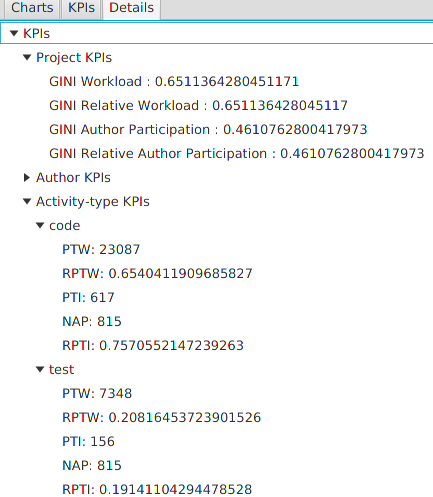
\includegraphics[width=.6\textwidth]{Project-mining-2-Mining-Type-of-Work/figures/brew3-cut}
    \caption{Detailed KPIs view of the \textsl{brew} project}
    \label{fig:brew3}
\end{figure}

\begin{figure}
    \centering
    \includegraphics[width=\textwidth]{Project-mining-2-Mining-Type-of-Work/figures/brew2-cut}
    \caption{Visualization of the effort distribution within the \textsl{brew} project}
    \label{fig:brew2}
\end{figure}

\begin{figure}
    \centering
    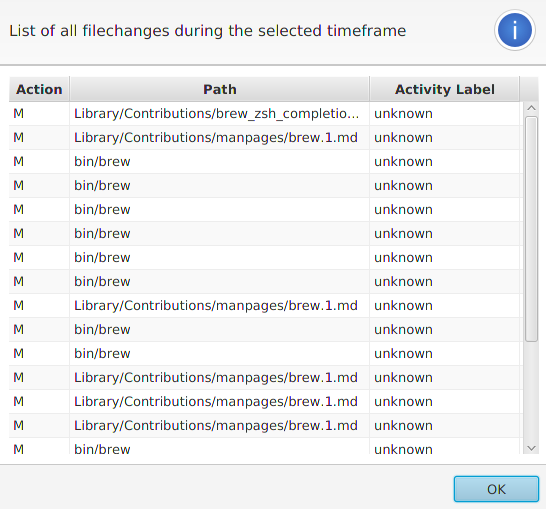
\includegraphics[width=.7\textwidth]{Project-mining-2-Mining-Type-of-Work/figures/brew1-cut}
    \caption{Details on file changes in the \textsl{brew} project}
    \label{fig:brew1}
\end{figure}

%\caption{ActiVCS applied on the real-life event log of the \textsl{brew} project}
%\label{fig:activcs-screenshots}
%\end{figure}

\Cref{fig:rup-phases,fig:brew3,fig:brew2,fig:brew1} show the visualization tool in action. We extracted the \gls{vcs} log of the \textsl{brew} project from GitHub. ActiVCS has a \gls{gui} with four main frames. The main frame is depicted in \Cref{fig:rup-phases}. It allows the domain expert to execute a number of actions. These actions are the following: \begin{inparaenum}[\itshape i)] 
\item load an event log; 
\item save an event log for reuse and avoid parsing it anew;
\item get help information;
\item change granularity of the timeline by choosing to display data daily, weekly or monthly; 
\item change data series on X-axis between commit-level and file-level; and
\item four buttons to change size and type of the plots.
\end{inparaenum}
The plots shown in the frame illustrate the evolution of the identified types of work over time. Through the drop-down menu on the left pane, the user can choose between showing the classification of the activity on a commit-level or on file-level.  

It is possible to interact with each point on the plot shown in the main frame. Depending whether the X-axis is showing the information at commit-level or at file-level, a pop-up menu that summarizes the information related to that point of the plot is shown. \Cref{fig:brew1} shows this pop-up window that lists the 20 changes corresponding to a select point of the plot, in which the X-axis was set at file-level. 
\Cref{fig:brew2} presents the main \glspl{kpi} on a pane with two bar-charts and some textual information below. The barchart on the left-hand-side shows the distribution of the workload by activity. The barchart on the right-hand-side shows the number of authors who participate on each activity (i.e., have worked at least once on that activity). The text in the middle provides \glspl{kpi} about the overall project. 
\Cref{fig:brew3} shows the information presented by the fourth frame. Here it is possible to obtain details on all the \glspl{kpi} about the users (e.g. on which activities they have worked on and how much), the overall-project (e.g., the distribution of workload) and the activities (e.g., how many different activities are in the project and what is the relative work done on them). 

With this information at hand and their knowledge of the domain, the project manager can investigate, for example whether the team is \textsl{de facto} following a specific software methodology.

\subsection{Analyses of real-life open-source projects}

We use ActiVCS to analyze real-life open source projects from GitHub. 
We chose thirteen projects of different size, age, user counts, and programming languages. Selection criteria included having, 
\begin{inparaenum}[\slshape i)]
\item a representative variety in terms of programming language,
\item variety in the size,
\item at least having two similar projects,
\item highly active versus inactive, and
\item fast versus slow growing projects.
\end{inparaenum}
 

This resulted in the following projects. 
\textsl{MPAndroidChart} \textsl{(MP} is a visualization library for Android platforms. 
\textsl{Torque2D} \textsl{(Torque)} is a software engine for the development of video games. 
\textsl{Openage (openage)}	is an open source clone of the Age of Empires II engine. 
\textsl{Incubator-dubbo} \textsl{(inc)}	is a RPC (remote procedure call) framework for Java. \textsl{jekyll}	is a blog-aware written Ruby that generates websites from user content. \textsl{scrapy} is a Python based framework to extract data from 24 websites
\textsl{brew} is a software that automatically installs missing packages for MacOS and Linux operating systems. 
\textsl{Algorithms -- Java} \textsl{(Java)} is a collection of different Java algorithms. 
\textsl{Flask (flask)} is a lightweight Web Server Gateway Interface (WSGI) web application framework created in Python. 
\textsl{Tablesaw} is a framework for the transformation and visualization of data, implemented in Java.
\textsl{Okhttp (ok)} is an HTTP client for Java and Android. 
\textsl{Retrotfit (retro)}	is another HTTP client for Java and Android.
\textsl{editor.js (editor)}	is a JavaScript based editor software for the creation of documents and the transformation into JSON format.

% Please add the following required packages to your document preamble:
% \usepackage{booktabs}
\begin{table}[h]
\caption{KPIs giving insights on real-life projects.}
\label{tab:kpis-results}
% \scriptsize
\centering
\begin{tabular}{@{}crrrrrrrrrr@{}}
\toprule
\textbf{Name} &
  \multicolumn{1}{c}{\textbf{COM}} &
  \multicolumn{1}{c}{\textbf{PW}} &
  \multicolumn{1}{c}{\textbf{NAP}} &
  \multicolumn{1}{c}{\textbf{NTP}} &
  \multicolumn{1}{c}{\textbf{PWS}} &
  \multicolumn{1}{c}{\textbf{PIS}} &
  \multicolumn{1}{c}{\textbf{C}} &
  \multicolumn{1}{c}{\textbf{D}} &
  \multicolumn{1}{c}{\textbf{T}} &
  \multicolumn{1}{c}{\textbf{U}} \\ \midrule
\textit{MP}       & 2012  & 8552  & 86   & 8  & 0.8  & 0.5  & 7352  & 53    & 24   & 351  \\
\textit{Torque}   & 970   & 7978  & 46   & 9  & 0.75 & 0.34 & 5410  & 134   & 241  & 1561 \\
\textit{openage}  & 3136  & 10529 & 168  & 9  & 0.74 & 0.5  & 7697  & 596   & 366  & 1126 \\
\textit{inc}      & 3308  & 31667 & 240  & 8  & 0.69 & 0.58 & 16116 & 6     & 8232 & 164  \\
\textit{jekyll}   & 10388 & 14369 & 1028 & 9  & 0.69 & 0.6  & 4085  & 1384  & 1492 & 7001 \\
\textit{scrapy}   & 7045  & 15014 & 409  & 9  & 0.68 & 0.57 & 7995  & 612   & 2784 & 525  \\
\textit{brew}     & 18410 & 35299 & 815  & 6  & 0.65 & 0.46 & 23087 & 1276  & 7348 & 3161 \\
\textit{Java}     & 755   & 902   & 175  & 5  & 0.65 & 0.58 & 636   & 5     & 7    & 203  \\
\textit{flask}     & 3505  & 5679  & 623  & 10 & 0.65 & 0.65 & 1950  & 206   & 1027 & 481  \\
\textit{tablesaw} & 1893  & 23700 & 39   & 7  & 0.63 & 0.39 & 8779  & 11149 & 2188 & 652  \\
\textit{ok}       & 3826  & 11567 & 245  & 7  & 0.63 & 0.51 & 5837  & 225   & 3348 & 260  \\
\textit{retro}    & 1721  & 5168  & 173  & 7  & 0.6  & 0.43 & 2467  & 69    & 1039 & 103  \\
\textit{editor}   & 494   & 2337  & 27   & 7  & 0.56 & 0.24 & 927   & 314   & 0    & 814  \\ \bottomrule
\end{tabular}
\end{table}

\Cref{tab:kpis-results} shows the KPIs resulting from these projects. Columns contain the following information: number of commits (COM), \glsfirst{pw}, \glsfirst{tw}, \glsfirst{nap}, \glsfirst{ntp}, \glsfirst{pws}, \glsfirst{pis}, code (C) , documentation (D) , testing (T) and unknown (U). Entries have been sorted by the \gls{pws}.  This means that, for instance, resources of project \textsl{MP} are highly occupied. Therefore, load balancing should be considered if the managers want to improve the capacity of the team to handle new tasks in the near future. 

Finally, the types of work code (C), documentation (D), testing (T) and unknown (U) that are displayed in the table make up the most frequently identified types that were detected with ActiVCS. As expected from software development processes, the main workload in most analyzed projects were coding activities.
One exception to this observation is the jekyll project. ActiVCS has detected
7001 file changes with an unknown type within the Ruby software application. Projects like these would provide a solid basis for the identification of
additional file types. The total amount of workload that was captured across all projects is 172761. The number of file changes which could not be classified by ActiVCS and were marked as unknown is 16402. This represents 9,49\% of the total workload. Excluding the jekyll project from the analysis would reduce this margin to 5,94\%. Many of the identified projects neglect the creation of documentation.
All of the analyzed projects with a workload value for coding activities of
8000 and more also have a noticeable amount of registered testing activities.
This could refer to the fact that large software development processes
have a need for automated test activities which must be frequently updated.
